\clearpage
\begin{column}{探索と活用のジレンマ（多腕バンディット問題の実験） - 長田晴人}

\ \textbf{実験設定と評価指標}\\
強化学習の重要なテーマの一つに，\textbf{探索と活用のジレンマ}がある．
ここでは，第\ssref{subsec:bandit}小節で取り上げた多腕バンディット問題を用いて，
いくつかの探索手法を同一条件で比較し，パラメータの違いが学習曲線に
どのように現れるかを確認する．

\ バンディット問題の名前は，スロットマシンが ``one-armed bandit''
と呼ばれていたことに由来する．
レバーを引くと確率的に報酬が得られるが，どのレバーの期待報酬が高いかは
プレイヤーには分からない．
本実験では，6本の腕 $a\in\{1,\ldots,6\}$ を持つバンディットを考え，
各腕を選ぶと確率
\[
    p=\left(\frac{1}{20},\frac{1}{10},\frac{1}{10},\frac{1}{10},\frac{1}{2},\frac{3}{4}\right)
\]
で報酬 $1$ が得られ，それ以外では報酬 $0$ が得られるとする．
学習者はこの真の確率を知らず，実際に得られた報酬から各腕の行動価値を推定する．
この問題では第6腕が最適腕であるが，第5腕も比較的高い報酬確率を持つため，
初期の偶然によって第5腕を過大評価し，第6腕を十分に試さないまま学習が進む可能性がある．

\ 比較する手法は，$\varepsilon$-greedy，softmax，UCB，optimistic 初期値，
Thompson sampling である．
このコラムの目的は，平均報酬と累積後悔の推移を通じて，
\textbf{探索の強さ}や\textbf{価値推定の方法}が学習過程に与える影響を観察することである．
確率的なばらつきを抑えるため，各条件について1000回の独立試行を行い，
その平均を学習曲線としてプロットする．

\ まず，行動価値の更新方法と腕の選択方法を分けて整理する．
表\ref{tab:bandit-value-update}は「得られた報酬をどのように価値推定へ反映するか」を表し，
表\ref{tab:bandit-action-selection}は「推定された価値にもとづいて次にどの腕を選ぶか」を表す．

\begin{center}
    \small
    \renewcommand{\arraystretch}{1.55}
    \captionof{table}{行動価値の更新方法}
    \label{tab:bandit-value-update}
    \begin{tabular}{p{0.42\linewidth}p{0.50\linewidth}}
      \toprule
      手法・式 & 備考 \\
      \midrule

      \textbf{標本平均手法}
      \[
      Q_t(a)
      =
      \frac{1}{N_t(a)}
      \sum_{\tau \leq t: A_\tau=a} r_\tau
      \]
      &
      $N_t(a)$ は，時刻 $t$ までに腕 $a$ を選んだ回数である．
      過去に腕 $a$ から得た報酬の平均をそのまま行動価値とする．
      定常環境では自然な推定方法であるが，過去の観測をすべて同じ重みで扱うため，
      非定常環境では古い情報を引きずりやすい．
      \\

      \midrule

      \textbf{逐次的な標本平均}
      \[
      Q_{t+1}(a)
      =
      Q_t(a)
      +
      \frac{1}{N_t(a)}
      \{r_t-Q_t(a)\}
      \]
      &
      標本平均手法を逐次更新の形で書いたものである．
      新しい報酬 $r_t$ と現在の推定値 $Q_t(a)$ の差を，
      選択回数の逆数だけ反映する．
      選択回数が増えるほど，新しい観測の影響は小さくなる．
      \\

      \midrule

      \textbf{固定学習率手法}
      \[
      Q_{t+1}(a)
      =
      Q_t(a)
      +
      \alpha\{r_t-Q_t(a)\}
      \]
      &
      $\alpha \in (0,1]$ は学習率である．
      新しい報酬を一定の重みで反映する方法であり，
      $\alpha$ が大きいほど最近の観測を重視し，小さいほど推定は安定する．
      標本平均手法と異なり，古い観測の影響が相対的に小さくなるため，
      非定常環境に追従しやすい．
      \\

      \bottomrule
    \end{tabular}
\end{center}

\begin{center}
    \small
    \renewcommand{\arraystretch}{1.55}
    \captionof{table}{多腕バンディット問題における腕の選択方法}
    \label{tab:bandit-action-selection}
    \begin{tabular}{p{0.42\linewidth}p{0.50\linewidth}}
      \toprule
      手法・式 & 備考 \\
      \midrule

      \textbf{greedy}
      \[
      A_t
      =
      \arg\max_{a\in\mathcal{A}} Q_t(a)
      \]
      &
      常に現在の推定価値 $Q_t(a)$ が最大の腕を選ぶ．
      探索を行わないため，初期の偶然によって悪い腕を過大評価すると，
      その腕を選び続ける可能性がある．
      \\

      \midrule

      \textbf{$\varepsilon$-greedy}
      \[
      A_t =
      \begin{cases}
      \arg\max\limits_{a\in\mathcal{A}} Q_t(a),
      & \text{確率 } 1-\varepsilon,\\
      \text{ランダムな腕},
      & \text{確率 } \varepsilon
      \end{cases}
      \]
      &
      $\varepsilon \in [0,1]$ は探索率である．
      確率 $\varepsilon$ でランダム探索を行う．
      $\varepsilon$ が大きいほど未知の腕を試しやすいが，
      学習後も低報酬の腕を選ぶ確率が残る．
      $\varepsilon=0$ では greedy と一致する．
      \\

      \midrule

      \textbf{softmax}
      \[
      \Pr(A_t=a)
      =
      \frac{\exp(Q_t(a)/\tau)}
      {\sum_{b\in\mathcal{A}}\exp(Q_t(b)/\tau)}
      \]
      &
      $\tau>0$ は温度パラメータである．
      $\tau$ が大きいほど選択確率は一様に近づき，
      $\tau$ が小さいほど greedy に近づく．
      価値差をどの程度鋭く選択確率に反映するかを決めるスケールパラメータとして解釈できる．
      \\

      \midrule

      \textbf{UCB}
      \[
      A_t
      =
      \arg\max_{a\in\mathcal{A}}
      \left\{
      Q_t(a)
      +
      c\sqrt{\frac{\log t}{N_t(a)}}
      \right\}
      \]
      &
      $c>0$ は探索ボーナスの強さ，
      $N_t(a)$ は腕 $a$ の選択回数である．
      選択回数が少ない腕ほど第2項が大きくなるため，
      未探索の腕を体系的に試す．
      $c$ が大きいほど探索的になり，小さいほど現在の推定価値を重視する．
      \\

      \midrule

      \textbf{optimistic 初期値}
      \[
      Q_0(a)=Q_{\mathrm{init}}
      \qquad
      (Q_{\mathrm{init}}\text{ を大きく設定})
      \]
      &
      $Q_{\mathrm{init}}$ は初期行動価値である．
      行動選択規則そのものではなく，初期価値を高く置くことで探索を促す方法である．
      まだ試していない腕が楽観的に評価されるため，
      明示的なランダム探索を入れなくても複数の腕を試しやすい．
      \\

      \midrule

      \textbf{Thompson sampling}
      \[
      \tilde{\theta}_a \sim P_t(\theta_a),
      \qquad
      A_t=\arg\max_{a\in\mathcal{A}}\mu(a;\tilde{\theta}_a)
      \]
      &
      $P_t(\theta_a)$ は，腕 $a$ の報酬分布のパラメータ $\theta_a$ に関する事後分布である．
      各腕の事後分布からパラメータをサンプリングし，
      そのもとでの期待報酬 $\mu(a;\tilde{\theta}_a)$ が最大の腕を選ぶ．
      今回は Bernoulli 報酬なので，成功確率 $p_a$ の事後分布として
      ベータ分布 $\mathrm{Beta}(\alpha_a,\beta_a)$ を用いる．
      \\

      \bottomrule
    \end{tabular}
\end{center}

\ 累積後悔についても簡単に述べておく．
平均報酬が「どれだけ報酬を得られたか」を表すのに対し，
累積後悔は「最初から最適腕を知っていた場合に比べて，
どれだけ報酬を取り逃したか」を表す．
時刻 $t$ に選んだ腕を $A_t$，その真の報酬確率を $p_{A_t}$，
最適腕の報酬確率を $p^\ast=3/4$ とすると，時刻 $T$ までの累積後悔は
\[
    R_T=\sum_{t=1}^{T}\left(p^\ast-p_{A_t}\right)
\]
で定義される．
この指標を見ることで，探索のために低確率の腕を引いたコストや，
第5腕のような「そこそこ良い腕」に固定されたことによる損失を評価できる．

\begin{center}
  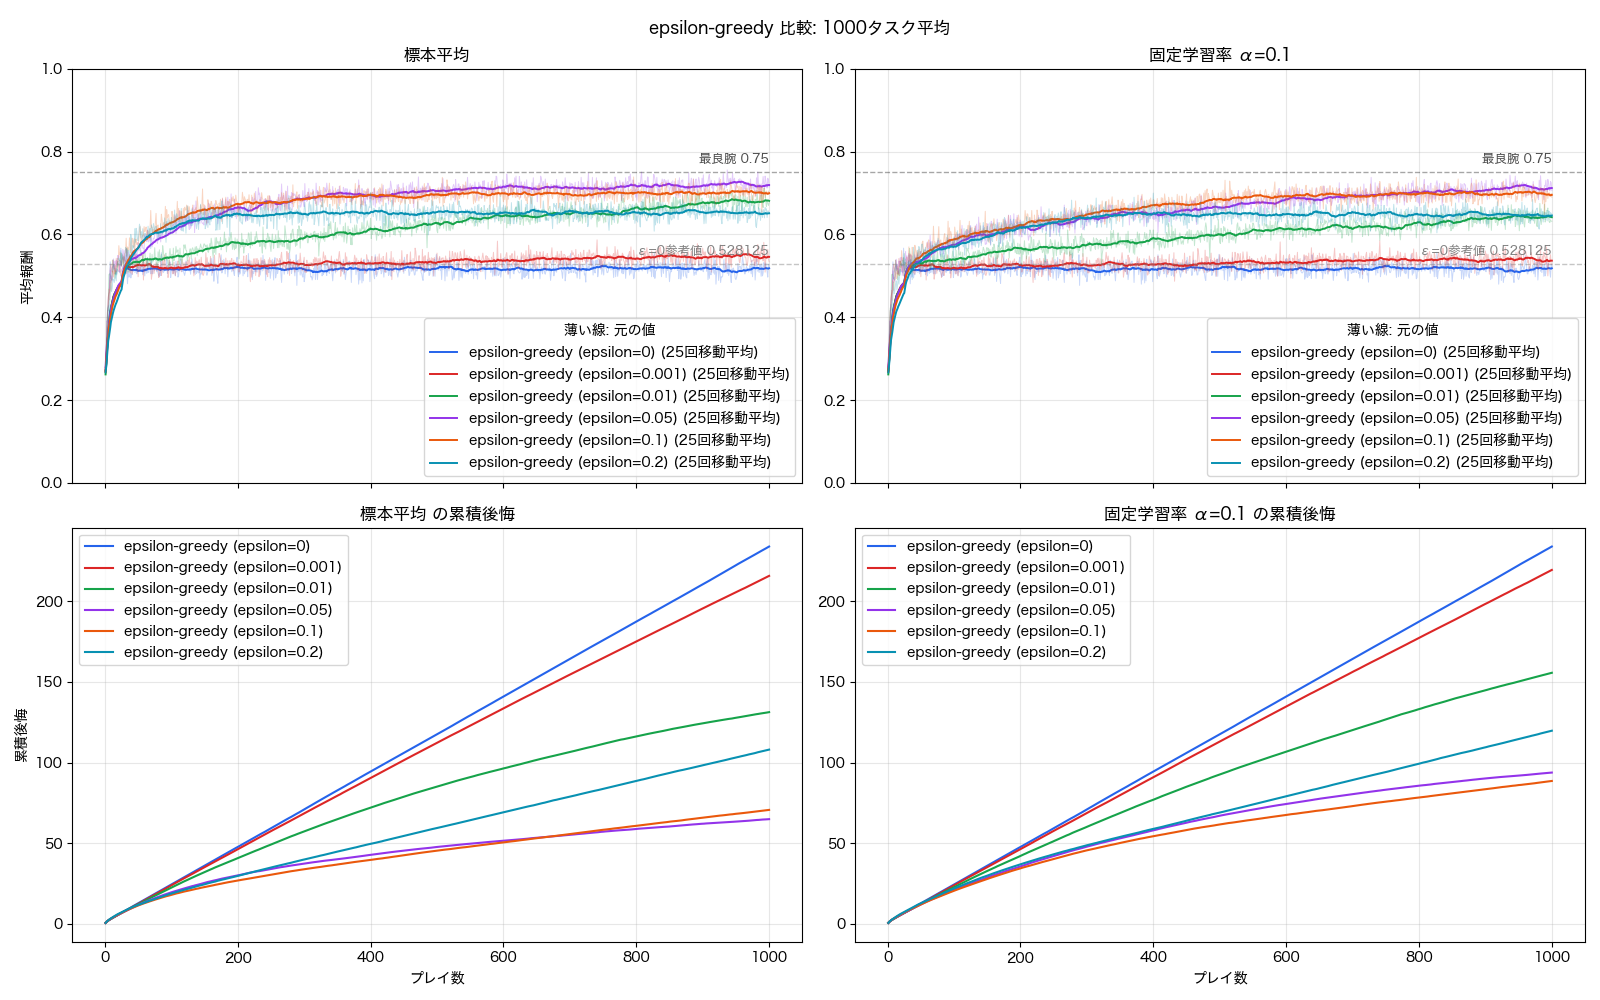
\includegraphics[width=\linewidth]{assets/reinforcement_column/greedy_graph.png}
  \captionof{figure}{greedy 法と $\varepsilon$-greedy 法の学習曲線}
  \label{fig:epsilon-greedy}
\end{center}

\ \textbf{greedy 法と $\varepsilon$-greedy 法}\\
図\ref{fig:epsilon-greedy}では，greedy 法と $\varepsilon$-greedy 法を比較した．
greedy 法は
\[
    A_t=\arg\max_{a\in\mathcal{A}}Q_t(a)
\]
により，常に現在の推定価値が最大の腕を選ぶ方法である．
一方，$\varepsilon$-greedy 法では，確率 $1-\varepsilon$ で greedy な腕を選び，
確率 $\varepsilon$ でランダムに腕を選ぶ．

\ $\varepsilon=0$ の greedy 法では，初期値をすべて $Q_0(a)=0$ とすると，
最初に報酬 $1$ を出した腕に固定されやすい．
報酬が出るまでは同点の腕をランダムに選ぶため，最初に成功する腕が $a$ である確率は
\[
    q_a=\frac{p_a}{\sum_{b=1}^{6}p_b}
\]
と近似できる．
したがって，長期的な平均報酬は
\[
    \bar{r}_{\infty}
    =
    \sum_{a=1}^{6}q_a p_a
    =
    \frac{\sum_{a=1}^{6}p_a^2}{\sum_{a=1}^{6}p_a}
\]
となる．
今回の設定では
\[
    \sum_{a=1}^{6}p_a=\frac{8}{5},
    \qquad
    \sum_{a=1}^{6}p_a^2=\frac{169}{200}
\]
であるから，
\[
    \bar{r}_{\infty}
    =
    \frac{169/200}{8/5}
    =
    \frac{169}{320}
    =
    0.528125
\]
となる．
これは図中の $\varepsilon=0$ の収束値とよく一致している．

\ 一方，$\varepsilon=0.2$ の場合，学習が十分進んで greedy 部分では第6腕を選べるようになったとしても，
全体の $20\%$ はランダムに腕を選ぶ．
このとき長期的な平均報酬はおよそ
\[
    (1-\varepsilon)p^\ast
    +
    \varepsilon \frac{1}{6}\sum_{a=1}^{6}p_a
\]
で与えられる．
今回の設定では $p^\ast=3/4$，
\[
    \frac{1}{6}\sum_{a=1}^{6}p_a
    =
    \frac{4}{15}
\]
であるから，
\[
    (1-0.2)\cdot\frac{3}{4}
    +
    0.2\cdot\frac{4}{15}
    \simeq
    0.653
\]
となる．
図で $\varepsilon=0.2$ の平均報酬が最適腕の $0.75$ より低い値に落ち着くのは，
学習後も一定確率で低報酬の腕を選び続けるためである．
つまり，\textbf{$\varepsilon$ は小さすぎても大きすぎてもよくない}．
今回の結果では，$\varepsilon=0.05$ から $0.1$ 程度が，
初期探索と後半の活用のバランスがよかった．

\ 累積後悔のグラフは，この違いを別の形で示している．
累積後悔の傾きは，各時刻でどれだけ報酬を取り逃しているか，すなわち瞬間的な後悔の大きさを表す．
たとえば，greedy 法が平均報酬 $\bar{r}_{\infty}$ の腕選択に固定されているとき，
累積後悔の傾きはおよそ
\[
    p^\ast-\bar{r}_{\infty}
\]
となる．
$\varepsilon=0$ では
\[
    \frac{3}{4}-0.528125=0.221875
\]
となり，後悔が大きな傾きで増え続ける．
これは，学習が速いというより，早い段階で誤った腕に固定されてしまっている状態である．

\ これに対して，$\varepsilon>0$ では初期に探索を行うため，序盤の累積後悔は増えやすい．
しかし，その探索によって最適腕を発見できれば，その後の累積後悔の傾きは小さくなる．
また，累積後悔の傾きが時間とともに小さく変化し続けている場合には，
腕の選択がまだ改善しており，学習が継続していると解釈できる．
逆に，累積後悔がほぼ直線になった場合には，腕の選択傾向がほぼ固定され，
その時点の方策で一定の損失を出し続けていると考えられる．
これは，初期に損をしてでも正しい腕を見つける「学習の速さ」と，
学習後に不要な探索をどれだけ減らせるかという「最終的な正確性」のトレードオフを表している．

\begin{center}
  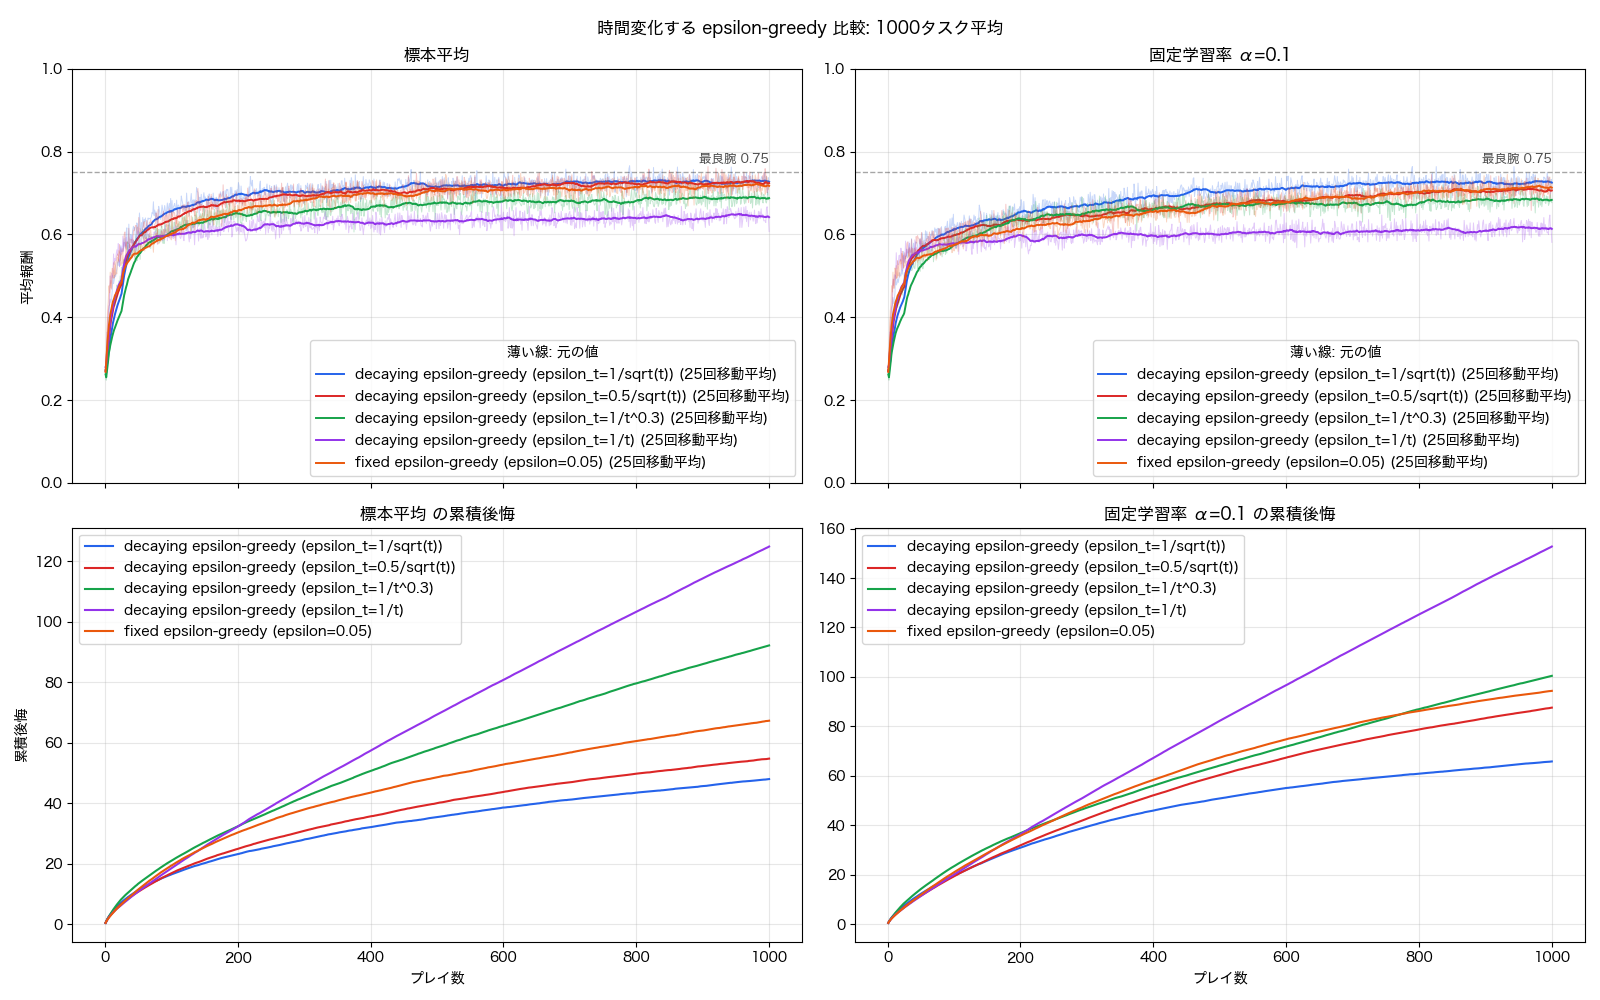
\includegraphics[width=\linewidth]{assets/reinforcement_column/time_greedy.png}
  \captionof{figure}{$\varepsilon$が時間変化する場合の学習曲線}
  \label{fig:decaying-epsilon-greedy}
\end{center}

\ \textbf{時間変化する $\varepsilon_t$-greedy 法}\\
固定した $\varepsilon$ を用いる $\varepsilon$-greedy 法では，
$\varepsilon$ が小さすぎると探索が不足し，初期に高く評価された腕に固定されやすい．
一方で，$\varepsilon$ が大きすぎると，最適腕を見つけた後もランダム探索が残り，
低報酬の腕を選ぶ損失が続いてしまう．
そこで，学習初期には十分に探索し，学習後半では不要な探索を減らすために，
時間とともに探索率を小さくする $\varepsilon_t$-greedy 法を考える．

\ $\varepsilon_t$-greedy 法では，
\[
    A_t =
    \begin{cases}
    \displaystyle \arg\max_{a\in\mathcal{A}} Q_t(a), & \text{確率 } 1-\varepsilon_t,\\
    \text{ランダムな腕}, & \text{確率 } \varepsilon_t
    \end{cases}
\]
として，各時刻 $t$ における探索率 $\varepsilon_t$ を変化させる．
本実験では，
\[
    \varepsilon_t=\frac{1}{\sqrt{t}},\quad
    \varepsilon_t=\frac{0.5}{\sqrt{t}},\quad
    \varepsilon_t=\frac{1}{t^{0.3}},\quad
    \varepsilon_t=\frac{1}{t}
\]
を比較し，固定値 $\varepsilon=0.05$ の場合とも比べた．

\ 図\ref{fig:decaying-epsilon-greedy}を見ると，
$\varepsilon_t=1/\sqrt{t}$ は，平均報酬と累積後悔の両方で比較的良い挙動を示している．
これは，時刻 $T$ までに発生するランダム探索の期待回数から説明できる．
$\varepsilon_t$-greedy 法では，各時刻に確率 $\varepsilon_t$ で探索を行うため，
探索回数 $M_T$ の期待値は
\[
    \mathbb{E}[M_T]
    =
    \sum_{t=1}^{T}\varepsilon_t
\]
である．
腕の本数を $K=6$ とすると，ランダム探索だけで各腕が試される回数の目安は
\[
    \frac{1}{K}\sum_{t=1}^{T}\varepsilon_t
\]
となる．

\ $\varepsilon_t=1/t$ の場合，
\[
    \sum_{t=1}^{T}\frac{1}{t}
    \simeq
    \log T
\]
である．
今回の実験では $T=1000$ なので，$\log 1000 \simeq 6.9$ となり，
各腕をランダム探索で試す回数は平均して1回程度にすぎない．
そのため，早い段階で探索率が小さくなりすぎ，
第6腕を十分に試す前に別の腕へ固定されやすい．

\ 一方，$\varepsilon_t=1/\sqrt{t}$ の場合，
\[
    \sum_{t=1}^{T}\frac{1}{\sqrt{t}}
    \simeq
    2\sqrt{T}
\]
である．
$T=1000$ では $2\sqrt{1000}\simeq 63$ となるため，
各腕はランダム探索だけでも平均して10回程度試される．
今回の報酬確率では，第6腕の報酬確率 $p_6=3/4$ と第5腕の報酬確率 $p_5=1/2$ の差が
\[
    \Delta=p_6-p_5=\frac{1}{4}
\]
と比較的大きい．
そのため，各腕を十数回程度試せば，第6腕が有望であることを発見するきっかけを得やすい．
さらに，$\varepsilon_t=1/\sqrt{t}$ は時間とともに $0$ に近づくため，
最適腕を見つけた後には不要なランダム探索が減り，平均報酬を高く保ちやすい．

\ これに対して，$\varepsilon_t=1/t^{0.3}$ の場合，
\[
    \sum_{t=1}^{T}\frac{1}{t^{0.3}}
    \simeq
    \frac{T^{0.7}}{0.7}
\]
であり，$T=1000$ ではおよそ $180$ 程度になる．
これは $\varepsilon_t=1/\sqrt{t}$ よりも探索回数が多く，
最適腕を発見するうえでは有利である．
しかし，学習後半にもランダム探索が多く残るため，
低報酬の腕を引く損失が続き，累積後悔の増加を抑えにくい．
つまり，$1/t$ は探索が減るのが速すぎ，$1/t^{0.3}$ は探索が残りすぎる．
その中間にある $1/\sqrt{t}$ は，今回の設定では
\textbf{探索不足と探索過多のバランス}がよかったと考えられる．

\ ここで，標本平均と固定学習率の違いにも注目したい．
固定した $\varepsilon$ の実験では両者の差は比較的小さかったが，
時間変化する $\varepsilon_t$ ではその差がより現れている．
標本平均手法では
\[
    Q_{t+1}(a)
    =
    Q_t(a)
    +
    \frac{1}{N_t(a)}\{r_t-Q_t(a)\}
\]
であり，腕 $a$ を多く選ぶほど新しい報酬の重み $1/N_t(a)$ は小さくなる．
一方，固定学習率では
\[
    Q_{t+1}(a)
    =
    Q_t(a)
    +
    \alpha\{r_t-Q_t(a)\}
\]
であり，新しい報酬は常に重み $\alpha$ で反映される．
実際，固定学習率の更新を展開すると
\[
    Q_n
    =
    (1-\alpha)^nQ_0
    +
    \sum_{i=1}^{n}\alpha(1-\alpha)^{n-i}r_i
\]
となり，最近の報酬ほど大きな重みを持つことが分かる．

\ 時間変化する $\varepsilon_t$ では，学習後半の探索機会が減るため，
後から得られた少数の観測をどれだけ強く価値推定に反映できるかが重要になる．
そのため，過去の観測を均等に平均する標本平均よりも，
最近の結果を大きく見る固定学習率の方が，減衰スケジュールの違いに敏感に反応しやすい．
このため，固定 $\varepsilon$ では目立たなかった価値更新方法の違いが，
時間変化する $\varepsilon_t$ の実験ではよりはっきり現れたと考えられる．

\ ただし，この結果は $\varepsilon_t=1/\sqrt{t}$ が一般に最適な減衰率であることを意味しない．
適切な減衰率は，腕の本数，プレイ回数，最適腕と次善腕の報酬確率差，
および価値更新方法に依存する．
今回の6本腕バンディット問題では，$T=1000$ という有限時間の中で，
$1/\sqrt{t}$ が「十分に探索するが，探索し続けすぎない」スケールになっていたと解釈できる．

\begin{center}
  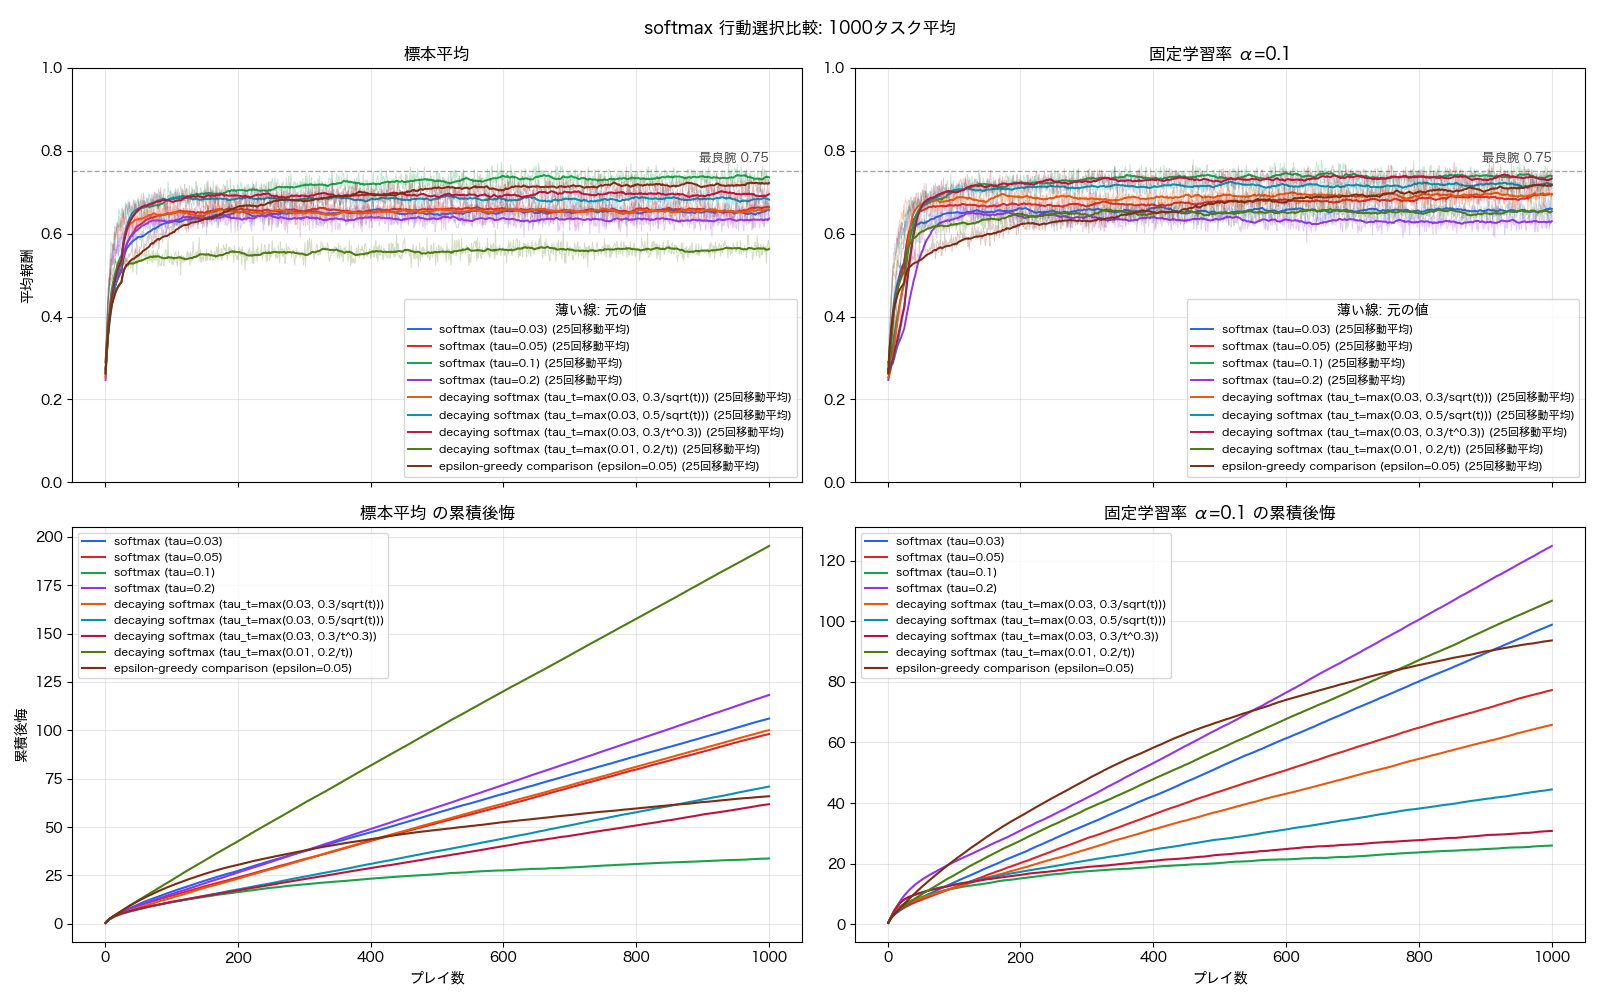
\includegraphics[width=\linewidth]{assets/reinforcement_column/softmax.png}
  \captionof{figure}{softmax 法の学習曲線}
  \label{fig:softmax}
\end{center}

\ \textbf{softmax 法}\\
次に，softmax による行動選択を比較する．
softmax 法では，各腕の推定行動価値 $Q_t(a)$ に対して
\[
    \Pr(A_t=a)
    =
    \frac{\exp(Q_t(a)/\tau)}
    {\sum_{b\in\mathcal{A}}\exp(Q_t(b)/\tau)}
\]
によって選択確率を与える．
ここで $\tau>0$ は温度パラメータであり，
$\tau$ が大きいほど各腕の選択確率は一様に近づき，
$\tau$ が小さいほど greedy 法に近づく．
したがって，$\tau$ は「価値の差をどれくらい鋭く行動選択に反映するか」を決める
スケールパラメータである．

\ 固定温度の結果を見ると，今回の設定では $\tau=0.1$ 付近が比較的よい性能を示している．
この理由は，今回の真の報酬確率の差の大きさから説明できる．
最適腕である第6腕と次善腕である第5腕の報酬確率差は
\[
    p_6-p_5
    =
    \frac{3}{4}-\frac{1}{2}
    =
    \frac{1}{4}
\]
である．
softmax では，2つの腕 $a,b$ の選択確率の比は
\[
    \frac{\Pr(A_t=a)}{\Pr(A_t=b)}
    =
    \exp\left(\frac{Q_t(a)-Q_t(b)}{\tau}\right)
\]
となる．
仮に推定値が真の報酬確率に近づき，
$Q_t(6)-Q_t(5)\simeq 0.25$ であるとすると，
$\tau=0.1$ のとき
\[
    \frac{\Pr(A_t=6)}{\Pr(A_t=5)}
    \simeq
    \exp\left(\frac{0.25}{0.1}\right)
    =
    \exp(2.5)
    \simeq 12.2
\]
となる．
つまり，第6腕は第5腕より十分選ばれやすいが，
第5腕が完全に排除されるほど極端でもない．
この程度の鋭さが，今回の問題では探索と活用のバランスとしてちょうどよかったと考えられる．

\ 一方，$\tau=0.2$ では
\[
    \exp\left(\frac{0.25}{0.2}\right)
    =
    \exp(1.25)
    \simeq 3.5
\]
となり，第6腕と第5腕の選択確率の差がそれほど大きくならない．
そのため，学習後も第5腕や他の腕を選ぶ確率が残りやすく，
平均報酬は最適値 $0.75$ から離れ，累積後悔も増えやすい．
逆に，$\tau=0.03$ のように温度が小さすぎると，
\[
    \exp\left(\frac{0.25}{0.03}\right)
    \simeq
    \exp(8.33)
\]
となり，わずかな価値差でも選択確率が極端に偏る．
学習が十分進んだ後であれば有利に働くが，
初期には $Q_t(a)$ の推定誤差が大きいため，
偶然高く評価された腕に選択が集中しやすい．

\ このように，softmax 法でも\textbf{温度は大きすぎても小さすぎてもよくない}．
今回の6本腕バンディット問題では，最適腕と次善腕の差が $0.25$ であるため，
$\tau=0.1$ 程度にすると
\[
    \frac{p_6-p_5}{\tau}
    =
    \frac{0.25}{0.1}
    =
    2.5
\]
となり，softmax の指数関数によって最適腕を十分に優遇しつつ，
完全な greedy にはならない程度の選択確率が得られる．
これが，固定温度 $\tau=0.1$ が今回うまく働いた主な理由である．

\ さらに，温度を時間とともに変化させる方法も試した．
これは，学習初期には温度を高めにして広く探索し，
学習が進むにつれて温度を下げることで，より価値の高い腕に選択を集中させる方法である．
本実験では，たとえば
\[
    \tau_t=\max\left(0.03,\frac{c}{\sqrt{t}}\right)
\]
のように，温度を減衰させつつ，下限値 $0.03$ を設けた．
下限を置いたのは，温度が小さくなりすぎるとほぼ greedy になり，
わずかな推定誤差にも過剰に反応してしまうためである．
図\ref{fig:softmax}では，温度を適切に減衰させた場合，
固定温度よりも累積後悔の増加を抑えられる場合がある．
これは，序盤では探索によって第6腕を発見する機会を確保し，
後半では温度低下によって第6腕への選択を強められるためである．

\begin{center}
  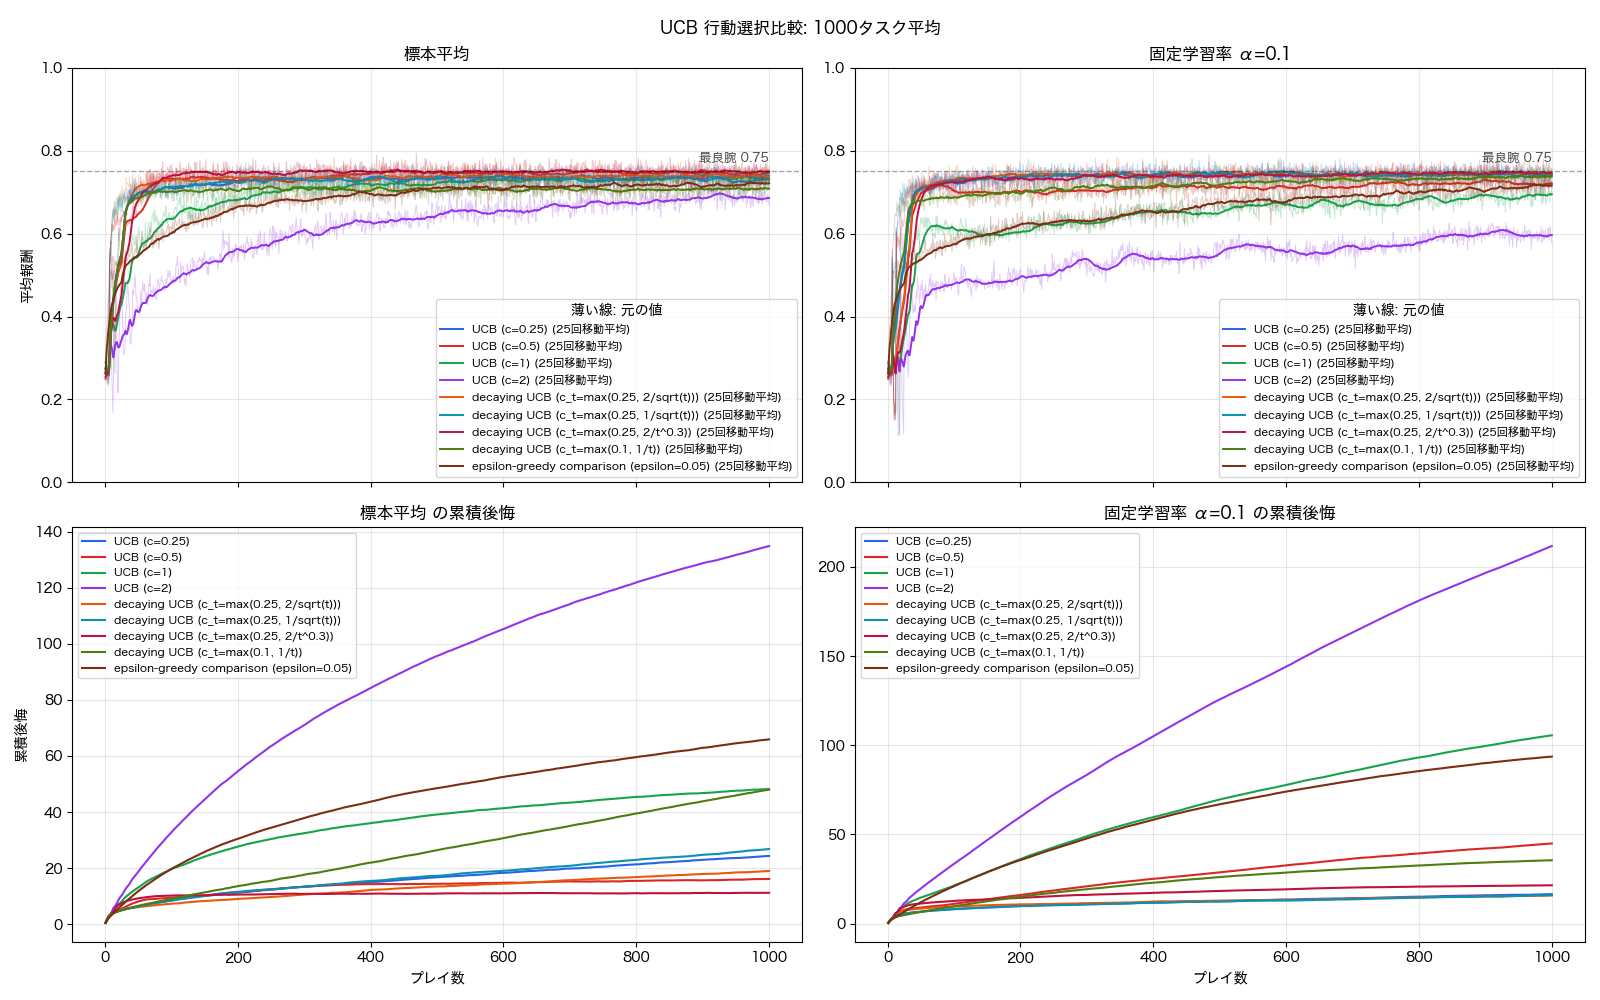
\includegraphics[width=\linewidth]{assets/reinforcement_column/ucb.png}
  \captionof{figure}{UCB 法の学習曲線}
  \label{fig:ucb}
\end{center}

\ \textbf{UCB 法}\\
次に，UCB による行動選択を比較する．
UCB は，現在の推定価値が高い腕だけでなく，
まだ十分に試されていない腕も高く評価する方法である．
具体的には，
\[
    A_t
    =
    \arg\max_{a\in\mathcal{A}}
    \left\{
        Q_t(a)
        +
        c\sqrt{\frac{\log t}{N_t(a)}}
    \right\}
\]
によって腕を選ぶ．
ここで $N_t(a)$ は時刻 $t$ までに腕 $a$ を選んだ回数であり，
$c>0$ は探索ボーナスの強さを決めるパラメータである．
第2項は，選択回数の少ない腕ほど大きくなるため，
UCB は単なるランダム探索ではなく，
\textbf{まだ不確実な腕を意図的に試す}方法と解釈できる．

\ 図\ref{fig:ucb}を見ると，$c$ が大きすぎる場合には性能が悪化している．
特に $c=2$ では平均報酬が低く，累積後悔も大きい．
これは，探索ボーナス
\[
    c\sqrt{\frac{\log t}{N_t(a)}}
\]
が大きすぎるために，すでに低報酬だと分かりつつある腕も繰り返し試してしまうからである．
今回の問題では，最適腕と次善腕の報酬確率差は
\[
    \Delta = p_6-p_5=\frac{1}{4}
\]
である．
したがって，探索ボーナスがこの差 $\Delta$ より十分大きい間は，
第6腕が高い推定価値を持っていても，試行回数の少ない腕が選ばれやすい．
つまり，$c$ が大きすぎると，UCB は慎重すぎる学習者になり，
不確実性を減らすための探索コストが累積後悔として残る．

\ 一方で，$c$ が小さい場合には，探索ボーナスが弱くなり，
現在の推定価値 $Q_t(a)$ をより重視する．
図では，$c=0.25$ や $c=0.5$ が比較的良い結果を示している．
これは，今回の6本腕バンディット問題では報酬確率の差が比較的大きく，
少ない試行回数でも第6腕の有利さを見つけやすかったためだと考えられる．

\ UCB の特徴は，累積後悔の傾きにも現れている．
$c$ が適切な場合，初期には全ての腕を試すために後悔が増えるが，
第6腕が有望であると分かるにつれて選択が集中し，
累積後悔の傾きが小さくなる．
一方，$c=2$ のように探索が強すぎる場合には，
後半になっても低報酬の腕を試す影響が残るため，
累積後悔の傾きが十分に小さくならない．

\ また，時間変化する UCB 係数 $c_t$ も比較した．
これは，学習初期には大きめの探索ボーナスで各腕を広く試し，
学習後半では探索ボーナスを小さくして，
推定価値の高い腕をより重視する方法である．
たとえば
\[
    c_t=\max\left(0.25,\frac{1}{\sqrt{t}}\right)
\]
のように設定すると，初期には強めに探索しつつ，
後半には $c_t$ が下限値 $0.25$ に近づく．
UCB の探索ボーナスそのものは
\[
    c_t\sqrt{\frac{\log t}{N_t(a)}}
\]
であるため，$c_t$ を小さくすることで後半の過剰な探索をさらに抑えられる．
ただし，$c_t$ を小さくしすぎると，
UCB の利点である「試行回数の少ない腕を体系的に試す」効果も弱くなる．
したがって，UCB でも探索の強さを問題のスケールに合わせることが重要である．

\begin{center}
  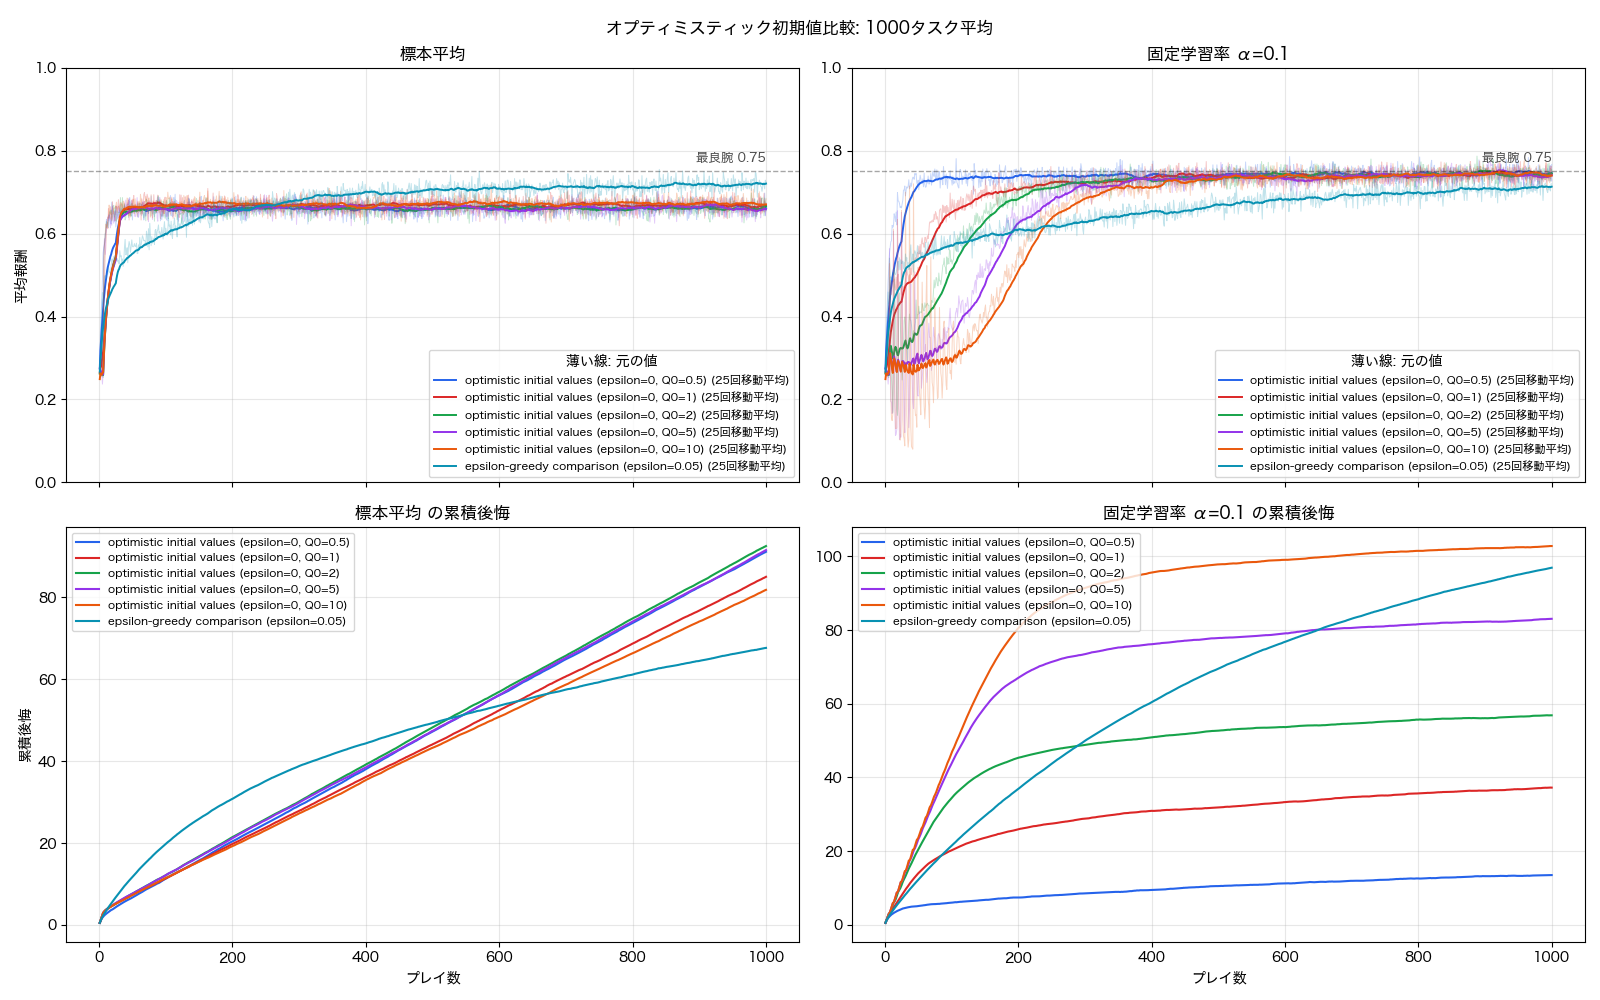
\includegraphics[width=\linewidth]{assets/reinforcement_column/optimistic.png}
  \captionof{figure}{オプティミスティック初期値の学習曲線}
  \label{fig:optimistic}
\end{center}

\ \textbf{optimistic 初期値}\\
次に，optimistic 初期値による探索を比較する．
これは，初期の行動価値 $Q_0(a)$ を高めに設定することで，
まだ十分に試していない腕を魅力的に見せる方法である．
本実験では $\varepsilon=0$ とし，明示的なランダム探索は行わず，
初期値の楽観性だけで探索がどの程度生じるかを調べた．

\ 図\ref{fig:optimistic}を見ると，標本平均を用いた場合には，
$Q_0$ を変えても最終的な結果はどれも似たように悪くなっている．
これは，標本平均手法では，腕 $a$ を初めて選んだ時点で
\[
    Q_1(a)=r_1
\]
となり，初期値 $Q_0(a)$ の影響がほとんど消えてしまうためである．
つまり，$Q_0$ をいくら大きくしても，その腕を一度試すと，
価値推定は実際に得られた $0$ または $1$ の報酬に置き換わる．
そのため，optimistic 初期値は「まだ一度も試していない腕を試させる」
効果は持つが，その後の価値推定には残りにくい．
結果として，標本平均では $Q_0$ の違いが学習曲線に大きく反映されず，
どの初期値でも似た挙動になったと考えられる．

\ 一方，固定学習率 $\alpha=0.1$ を用いた場合には，
初期値によって学習速度に大きな差が現れている．
固定学習率の更新は
\[
    Q_{n}(a)
    =
    (1-\alpha)^n Q_0(a)
    +
    \sum_{i=1}^{n}
    \alpha(1-\alpha)^{n-i}r_i
\]
と展開できる．
この式から分かるように，固定学習率では初期値の影響が
$(1-\alpha)^n Q_0(a)$ として残る．
したがって，$Q_0$ を大きくすると，その腕が何度か低い報酬を出しても，
しばらくは高く評価され続ける．

\ 図では，$Q_0=0.5$ の場合に平均報酬が早く高い値へ到達し，
累積後悔も小さくなっている．
これは，初期値が大きすぎず，初期の探索を促しつつ，
低報酬の腕への過大評価が比較的早く解消されたためだと考えられる．
逆に，$Q_0=5$ や $Q_0=10$ のように初期値が大きすぎると，
低報酬の腕も長い間高く評価され続ける．
たとえば報酬がしばらく $0$ だった場合，固定学習率では
\[
    Q_n(a)=(1-\alpha)^n Q_0(a)
\]
となる．
$\alpha=0.1$ では $(1-\alpha)^n=0.9^n$ なので，
$Q_0$ が大きいほど，その過大評価が十分に下がるまで多くの試行が必要になる．

\ 以上より，optimistic 初期値は，標本平均よりも固定学習率と組み合わせたときに
特徴が現れやすい．
標本平均では初期値が一度の観測でほぼ消えてしまうのに対し，
固定学習率では初期値の影響がしばらく残るため，
初期値の大きさが探索の強さと学習速度を大きく左右する．
ただし，初期値は大きければよいわけではなく，
小さすぎると探索を促せず，大きすぎると悪い腕への過大評価が長く残る．
今回の結果は，optimistic 初期値もまた，
問題の報酬スケールに合わせて設定する必要があることを示している．

\begin{center}
  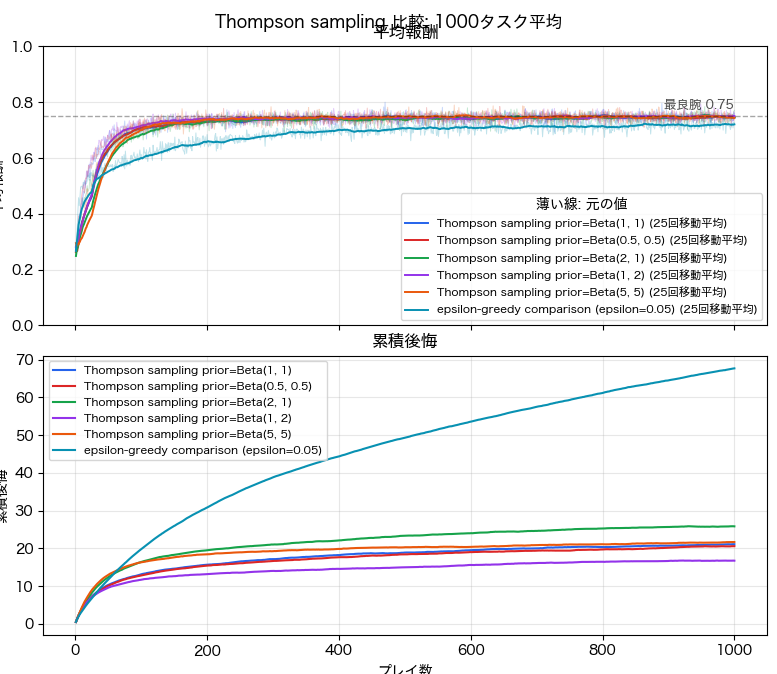
\includegraphics[width=\linewidth]{assets/reinforcement_column/thompson.png}
  \captionof{figure}{Thompson sampling の学習曲線}
  \label{fig:thompson}
\end{center}

\ \textbf{Thompson sampling}\\
最後に，Thompson sampling による行動選択を比較する．
Thompson sampling では，各腕の報酬確率そのものを一点推定するのではなく，
その不確実性を確率分布として保持する．
各時刻では，腕 $a$ の報酬確率に関する事後分布から値をサンプリングし，
そのサンプル値が最大となる腕を選ぶ．

\ 今回の実験では報酬が Bernoulli$(p_a)$ に従うため，
各腕の成功確率 $p_a$ に対してベータ分布を用いる．
時刻 $t$ における腕 $a$ の事後分布を
\[
    p_a \sim \mathrm{Beta}(\alpha_a,\beta_a)
\]
とし，そこから
\[
    \tilde{p}_a \sim \mathrm{Beta}(\alpha_a,\beta_a)
\]
をサンプリングして，
\[
    A_t=\arg\max_{a\in\mathcal{A}}\tilde{p}_a
\]
により腕を選ぶ．
報酬 $1$ が得られた場合は $\alpha_a$ を増やし，
報酬 $0$ が得られた場合は $\beta_a$ を増やす．
したがって，Thompson sampling では，探索は外から加えるランダム行動ではなく，
\textbf{報酬確率に関する不確実性}から自然に生じる．

\ 図\ref{fig:thompson}では，事前分布の違いによる学習曲線の変化を比較している．
ベータ分布 $\mathrm{Beta}(\alpha,\beta)$ の平均は
\[
    \mathbb{E}[p]
    =
    \frac{\alpha}{\alpha+\beta}
\]
であり，$\alpha+\beta$ が大きいほど事前分布は強くなる．
つまり，$(\alpha,\beta)$ は単なる初期値ではなく，
「はじめにどの程度の成功・失敗を仮想的に見たことにするか」を表している．

\ 結果を見ると，Thompson sampling は全体として
$\varepsilon$-greedy の比較対象よりも累積後悔が小さく，
平均報酬も早く高い値に近づいている．
これは，各腕の不確実性を分布として持つことで，
まだ情報が少ない腕には自然に探索の余地が残り，
成功が多く観測された腕には選択が集まりやすくなるためである．

\ 事前分布の違いに注目すると，
$\mathrm{Beta}(1,2)$ が特に小さい累積後悔を示している．
この事前分布の平均は $1/3$ であり，成功確率をやや低めに見積もる悲観的な事前分布である．
今回の問題では低報酬の腕が多いため，成功確率をやや低く見る事前分布は，
低報酬の腕を早めに見切る方向に働きやすい．
その一方で，第6腕のように成功が多く観測される腕では，
事後分布がすぐに高い値へ移動するため，選択が集中しやすい．

\ 一方，$\mathrm{Beta}(2,1)$ は平均 $2/3$ を持つ楽観的な事前分布である．
この場合，各腕の成功確率を初期には高めに見積もるため，
低報酬の腕についても「本当は良い腕かもしれない」という不確実性が残りやすい．
その結果，低報酬の腕を見切るまでにやや時間がかかり，
累積後悔が大きくなりやすい．
これは，optimistic 初期値において初期値を大きくしすぎると
悪い腕への過大評価が長く残ることと似ている．

\ また，$\mathrm{Beta}(0.5,0.5)$ は U 字型の分布であり，
成功確率が $0$ 付近または $1$ 付近にある可能性を比較的大きく見る事前分布である．
そのため，初期にはサンプル値が極端になりやすく，
不確実性に基づく探索がやや強く出る．
一方，$\mathrm{Beta}(5,5)$ は平均 $1/2$ の周辺に集中した事前分布であり，
初期にはどの腕も中程度の成功確率を持つという強めの信念を置く．
この場合，観測が少ない段階では事前分布の影響が残り，
第6腕の優位性を反映するまでに少し時間がかかる．

\ この結果から，Thompson sampling における事前分布は，
単なる初期設定ではなく，探索の性質そのものを決める要素であることが分かる．
中立的な事前分布では観測に素直に反応し，
楽観的な事前分布では探索が長く残りやすく，
悲観的な事前分布では低報酬の腕を早く見切りやすい．
ただし，悲観的すぎる事前分布では本当に良い腕を十分に試す前に
候補から外してしまう危険もあるため，事前分布も問題の報酬スケールに依存して調整される．

\begin{center}
  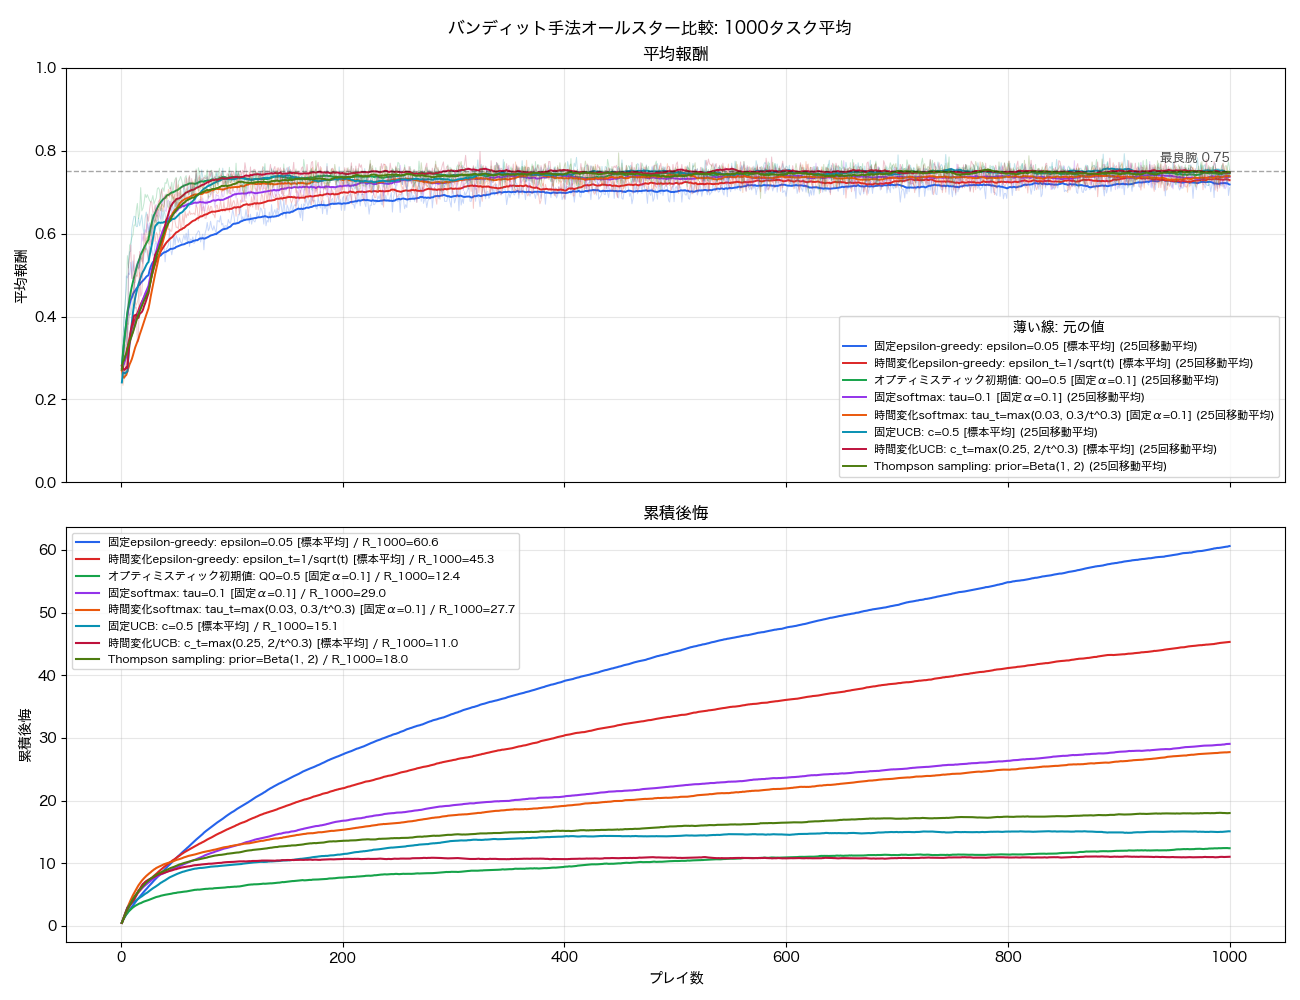
\includegraphics[width=\linewidth]{assets/reinforcement_column/allstar.png}
  \captionof{figure}{全手法の，最も累積後悔が小さくなるようなパラメータでの学習曲線}
  \label{fig:bandit-allstar}
\end{center}

\ \textbf{手法間の比較とまとめ}\\
最後に，各手法について今回の問題で比較的よい性能を示したパラメータを選び，
同一の図で比較した．
図\ref{fig:bandit-allstar}を見ると，平均報酬の推移だけでは，
多くの手法が最終的に最適腕の期待報酬 $0.75$ 付近へ近づいており，
大きな差は見えにくい．
しかし，累積後悔を見ると，各手法の違いはかなり明確に現れる．
これは，平均報酬が「最終的にどこまで到達したか」を見る指標であるのに対し，
累積後悔は「そこに至るまでにどれだけ損をしたか」を記録する指標だからである．

\ 今回の結果では，optimistic 初期値，時間変化する UCB，固定 UCB が特に小さい累積後悔を示している．
optimistic 初期値は，初期価値を高く設定することで未試行の腕を自然に試させるため，
初期の探索を素早く行うことができる．
今回のように定常的で，かつ最適腕と次善腕の差が比較的大きい問題では，
一度よい腕を見つければそのまま活用しやすく，累積後悔が小さくなったと考えられる．
また UCB は，試行回数の少ない腕に探索ボーナスを与えるため，
ランダムに探索するのではなく，不確実な腕を体系的に試すことができる．
その結果，探索の無駄が少なく，早い段階で第6腕へ選択を集中できたと解釈できる．

\ 一方で，固定 $\varepsilon$-greedy は累積後悔が大きくなっている．
これは，最適腕を見つけた後も確率 $\varepsilon$ でランダム探索を続けるためである．
学習が十分に進んだ後の平均報酬は
\[
    (1-\varepsilon)p^\ast
    +
    \varepsilon \frac{1}{K}\sum_{a=1}^{K}p_a
\]
で近似されるため，$\varepsilon>0$ である限り，
低報酬の腕を引く損失が残る．
時間変化する $\varepsilon_t$-greedy は，初期には探索し，
後半には $\varepsilon_t$ を小さくすることでこの問題を緩和している．

\ softmax でも，固定温度では学習後も確率的な選択が残る．
温度 $\tau$ が大きいと探索が残りすぎ，温度が小さいと初期の推定誤差に過敏になる．
今回の比較では，時間変化する softmax は固定 softmax よりよい結果を示しており，
温度を下げながら探索から活用へ移行することの有効性が見られる．
ただし，softmax は価値差を指数関数で選択確率に変換するため，
適切な温度スケールは報酬確率差に強く依存する．
今回うまくいった温度が，他の報酬スケールでもそのまま有効とは限らない．

\ Thompson sampling も比較的良い結果を示している．
探索率や温度を外から指定するのではなく，
各腕の報酬確率に関する事後分布からサンプリングすることで探索が生じるため，
明示的な探索率を設定しなくても，探索と活用のバランスを比較的うまく取ることができたと考えられる．

\ ただし，ここまでの結果は\textbf{定常バンディット問題}における比較である．
各腕の真の報酬確率 $p_a$ が時刻によらず一定であるという仮定のもとでは，
過去の観測を蓄積することに意味があり，
標本平均，UCB，Thompson sampling のように，
観測回数が増えるほど推定を確信していく手法が有効に働きやすい．
しかし，非定常環境では古い観測が現在の環境を表さない可能性がある．
そのため，過去の全データを同じ重みで用いる標本平均手法は，
変化後の最適腕に追従しにくい．

\ この観点から見ると，定常環境で特に意味を持つ手法と，
非定常環境でも活かしやすい手法を分けて考える必要がある．
標本平均に基づく greedy，UCB，通常の Thompson sampling は，
基本的には「真の報酬確率が一定であり，観測を重ねるほど正しい値に近づく」
という考え方に支えられている．
したがって，定常環境では強いが，非定常環境では古い情報を信じすぎる危険がある．
特に UCB では，ある腕を十分に試した後は探索ボーナス
\[
    c\sqrt{\frac{\log t}{N_t(a)}}
\]
が小さくなるため，環境変化後にその腕を再び探索する力は弱くなる．
Thompson sampling でも，観測数が増えて事後分布が鋭くなると，
過去の信念が強く残り，新しい変化に反応しにくくなる場合がある．

\ 一方，固定学習率による価値更新や，探索率・温度・UCB係数を時間変化させる設計は，
非定常環境へ拡張する余地を持つ．
固定学習率では
\[
    Q_n
    =
    (1-\alpha)^nQ_0
    +
    \sum_{i=1}^{n}\alpha(1-\alpha)^{n-i}r_i
\]
となり，最近の報酬ほど大きな重みを持つ．
したがって，古い観測を徐々に忘れながら，新しい環境に追従しやすい．
同様に，非定常環境では探索率を完全には下げきらず，
一定の探索を残すことにも意味がある．
定常環境では不要な探索は後悔を増やすが，
非定常環境では，環境変化を発見するための観測機会になるからである．

\ 以上の比較から，多腕バンディット問題における手法の良し悪しは，
単に平均報酬の高さだけでは判断できないことが分かる．
それぞれの違いは，最適腕をどれだけ早く見つけるか，
低報酬の腕をどれだけ早く見切るか，
そして学習後に不要な探索をどれだけ残すかという形で，
累積後悔の曲線に現れる．

\ 本実験を通じて，多腕バンディット問題は，
強化学習における探索と活用を理解するための最小構成の実験場であることが確認できた．
状態遷移を持たない単純な問題であっても，
探索率，温度，探索ボーナス，初期値，事前分布，学習率の選び方によって，
学習曲線は大きく変化する．
したがって，より複雑な強化学習問題を扱う際にも，
アルゴリズムを名前で選ぶのではなく，
その手法が\textbf{何を不確実とみなし，どのように探索し，どの程度過去を信じるのか}
を考えることが重要である．

\end{column}
\clearpage
